\documentclass[10pt]{article}
\usepackage[T1]{fontenc}
\usepackage[letterpaper,landscape,margin=0.22in]{geometry}
\usepackage{tgbonum}
\usepackage[dvipsnames]{xcolor}
\usepackage{tikz}
\usetikzlibrary{calc}

\pagestyle{empty}
\setlength{\parindent}{0pt}

\definecolor{AidInk}{HTML}{17212B}
\definecolor{AidGray}{HTML}{E9EDF0}
\definecolor{AidLight}{HTML}{F7F8F9}
\definecolor{EconomyGreen}{HTML}{39745A}
\definecolor{EconomyPale}{HTML}{E3F0E8}
\definecolor{FleetBlue}{HTML}{376E8C}
\definecolor{FleetPale}{HTML}{E1EDF3}

\begin{document}
\centering
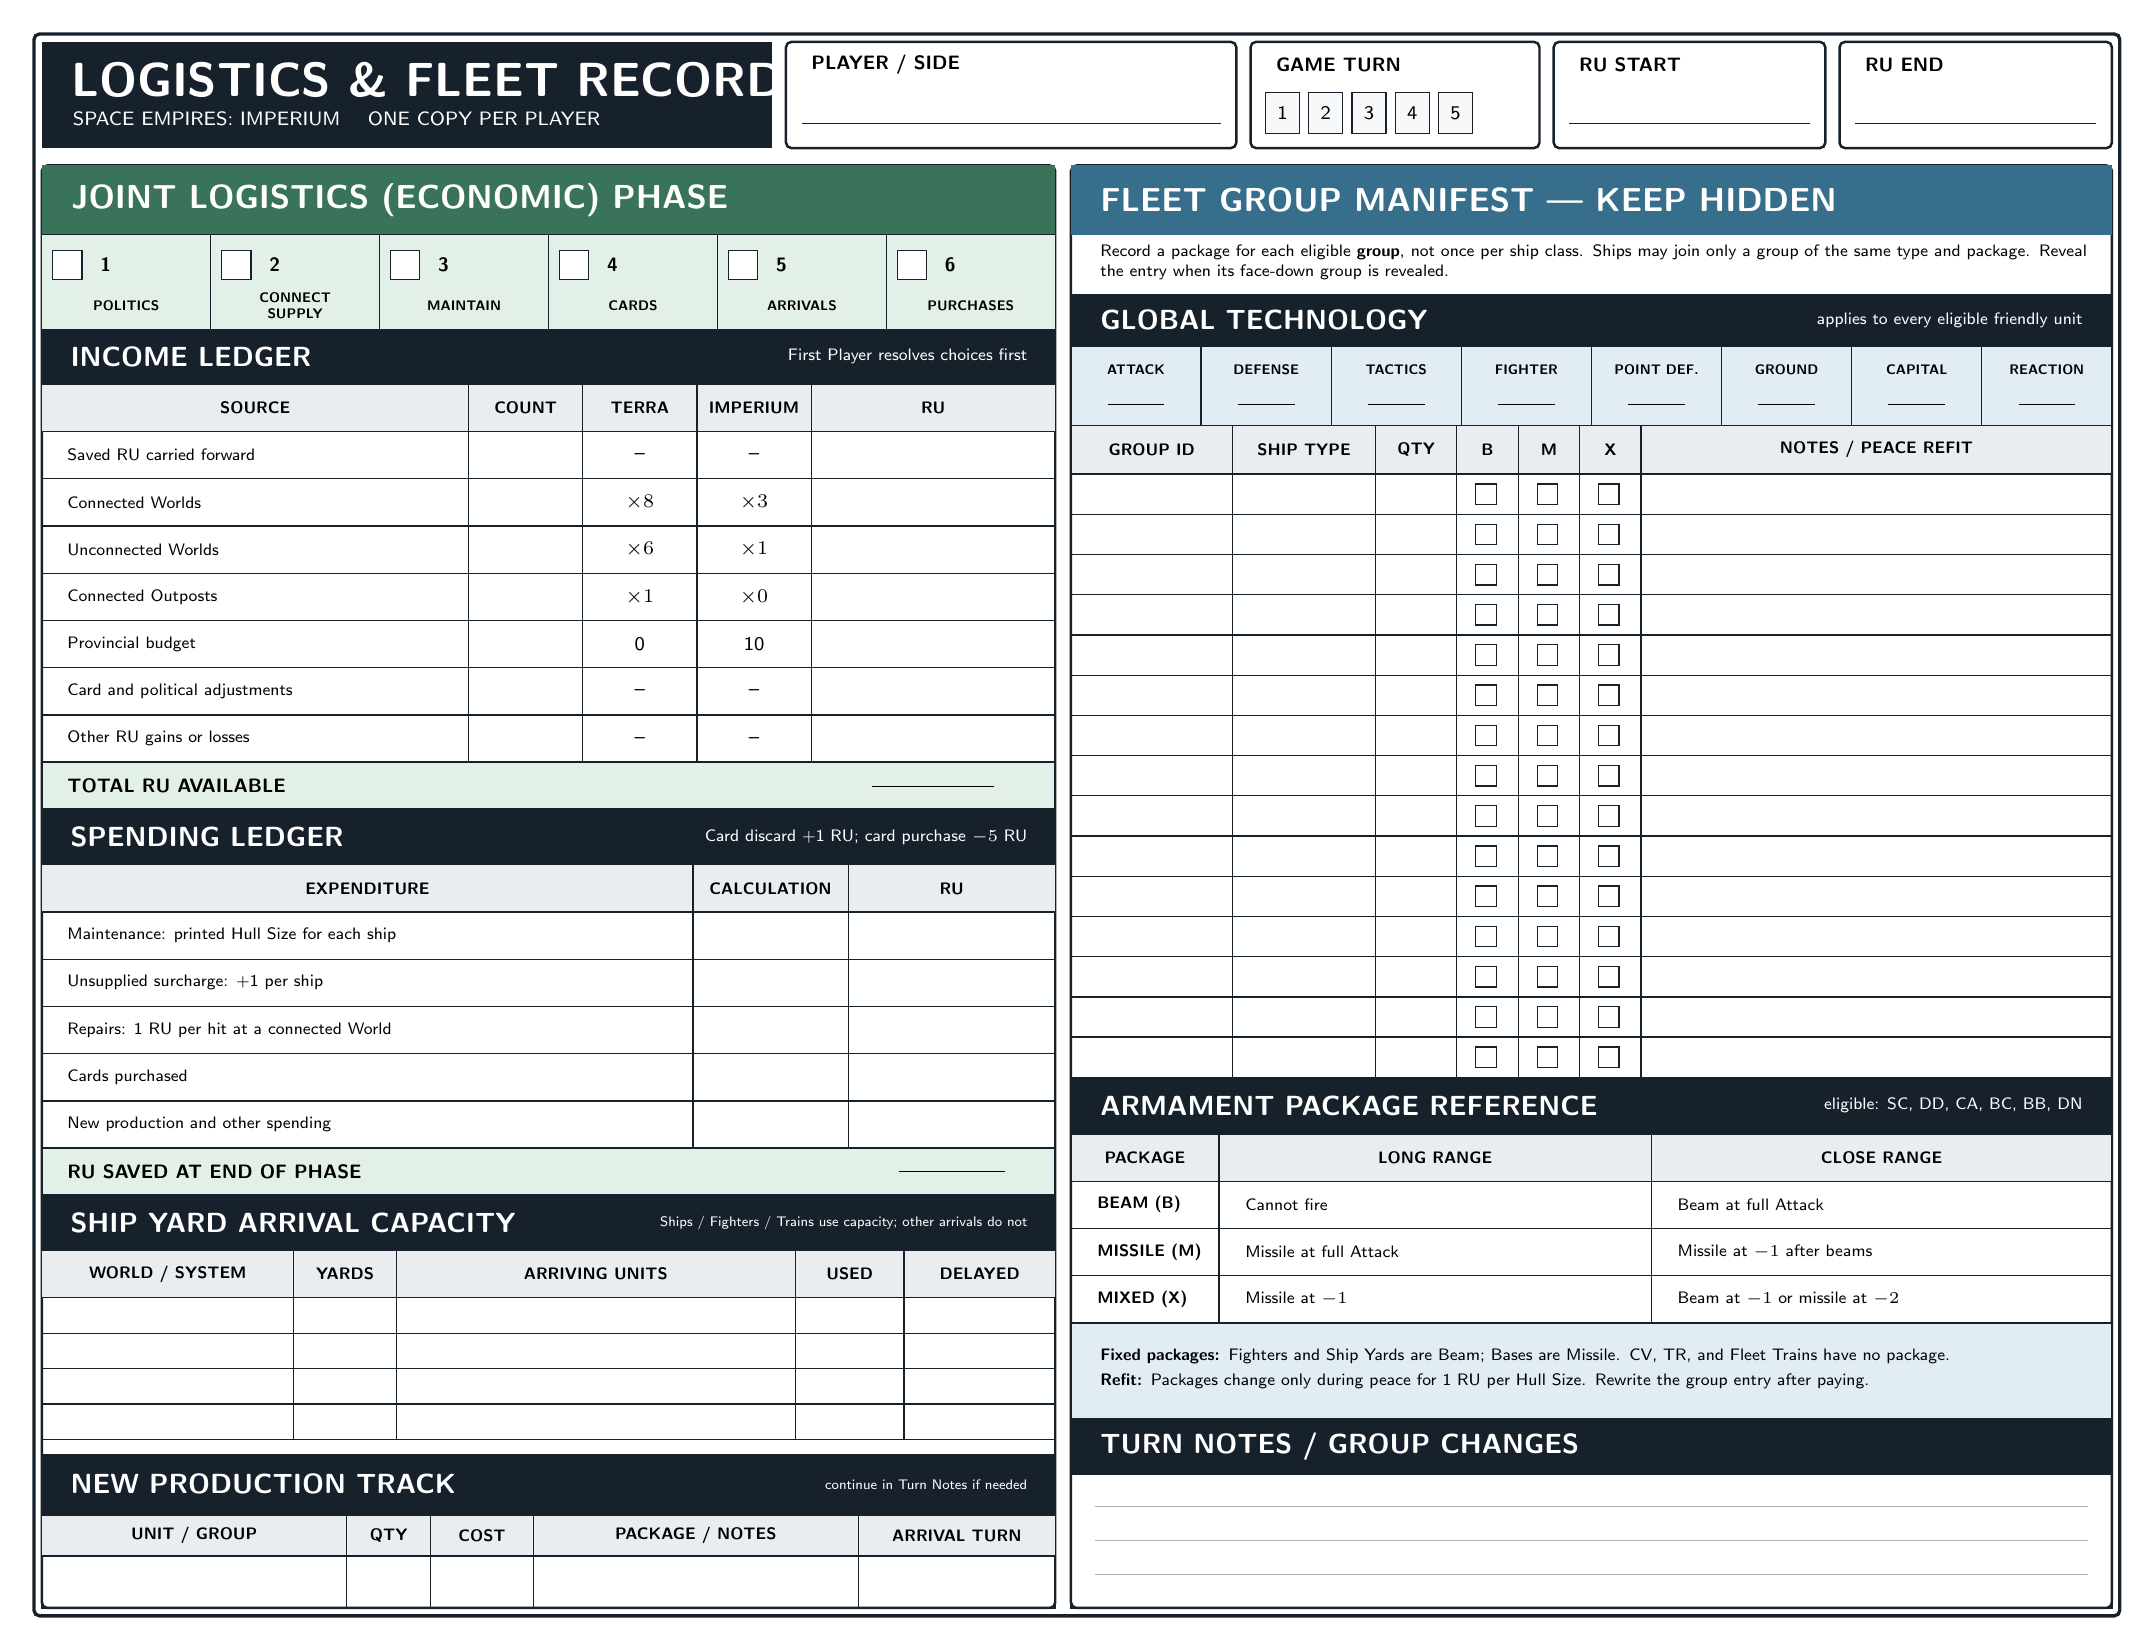
\begin{tikzpicture}[
  x=1cm,y=1cm,
  outer/.style={draw=AidInk,line width=0.9pt,rounded corners=2pt},
  rule/.style={draw=AidInk,line width=0.45pt},
  label/.style={font=\bfseries\sffamily\scriptsize},
  tinylabel/.style={font=\bfseries\sffamily\fontsize{5.6}{6.2}\selectfont},
  note/.style={font=\sffamily\fontsize{6.2}{7.1}\selectfont,align=left},
  micronote/.style={font=\sffamily\fontsize{5.6}{6.3}\selectfont,align=left},
  cell/.style={font=\sffamily\fontsize{6.4}{7.1}\selectfont,align=left},
  centertext/.style={font=\sffamily\scriptsize,align=center}
]
  \path[use as bounding box] (0,0) rectangle (26.65,20.25);
  \draw[outer,line width=1.2pt] (0.08,0.08) rectangle (26.57,20.17);

  % Header
  \fill[AidInk] (0.18,18.72) rectangle (9.45,20.07);
  \node[anchor=west,text=white,font=\bfseries\sffamily\LARGE]
    at (0.43,19.59) {LOGISTICS \& FLEET RECORD};
  \node[anchor=west,text=white,font=\sffamily\scriptsize]
    at (0.45,19.09) {SPACE EMPIRES: IMPERIUM \quad ONE COPY PER PLAYER};

  \draw[outer] (9.63,18.72) rectangle (15.35,20.07);
  \node[label,anchor=west] at (9.83,19.78) {PLAYER / SIDE};
  \draw[rule] (9.83,19.03) -- (15.15,19.03);

  \draw[outer] (15.53,18.72) rectangle (19.20,20.07);
  \node[label,anchor=west] at (15.73,19.78) {GAME TURN};
  \foreach \n [count=\i from 0,evaluate=\i as \x using 15.72+0.55*\i]
    in {1,2,3,4,5} {
    \draw[rule,fill=AidLight] (\x,18.91) rectangle +(0.43,0.52);
    \node[centertext] at ($(\x,18.91)+(0.215,0.26)$) {\n};
  }

  \draw[outer] (19.38,18.72) rectangle (22.83,20.07);
  \node[label,anchor=west] at (19.58,19.78) {RU START};
  \draw[rule] (19.58,19.03) -- (22.63,19.03);

  \draw[outer] (23.01,18.72) rectangle (26.47,20.07);
  \node[label,anchor=west] at (23.21,19.78) {RU END};
  \draw[rule] (23.21,19.03) -- (26.27,19.03);

  % Left: logistics worksheet
  \draw[outer] (0.18,0.18) rectangle (13.05,18.50);
  \fill[EconomyGreen] (0.18,17.62) rectangle (13.05,18.50);
  \node[anchor=west,text=white,font=\bfseries\sffamily\large]
    at (0.43,18.06) {JOINT LOGISTICS (ECONOMIC) PHASE};

  % Six-step checklist
  \foreach \i/\num/\txt in {
    0/1/POLITICS,
    1/2/CONNECT\\SUPPLY,
    2/3/MAINTAIN,
    3/4/CARDS,
    4/5/ARRIVALS,
    5/6/PURCHASES} {
    \pgfmathsetmacro{\xa}{0.18+2.145*\i}
    \pgfmathsetmacro{\xb}{0.18+2.145*(\i+1)}
    \draw[rule,fill=EconomyPale] (\xa,16.42) rectangle (\xb,17.62);
    \draw[rule,fill=white] ({\xa+0.14},17.05) rectangle +(0.37,0.37);
    \node[anchor=west,font=\bfseries\sffamily\scriptsize]
      at ({\xa+0.62},17.235) {\num};
    \node[font=\bfseries\sffamily\fontsize{5.4}{6.0}\selectfont,align=center]
      at ({(\xa+\xb)/2},16.72) {\txt};
  }

  % Income ledger
  \fill[AidInk] (0.18,15.72) rectangle (13.05,16.42);
  \node[anchor=west,text=white,font=\bfseries\sffamily\normalsize]
    at (0.42,16.07) {INCOME LEDGER};
  \node[anchor=east,text=white,font=\sffamily\fontsize{6}{6.8}\selectfont]
    at (12.82,16.07) {First Player resolves choices first};

  \def\ixA{0.18}\def\ixB{5.60}\def\ixC{7.05}\def\ixD{8.50}
  \def\ixE{9.95}\def\ixF{13.05}
  \draw[rule,fill=AidGray] (\ixA,15.12) rectangle (\ixF,15.72);
  \foreach \x in {\ixB,\ixC,\ixD,\ixE} {\draw[rule] (\x,10.92) -- (\x,15.72);}
  \node[tinylabel] at (2.89,15.42) {SOURCE};
  \node[tinylabel] at (6.325,15.42) {COUNT};
  \node[tinylabel] at (7.775,15.42) {TERRA};
  \node[tinylabel] at (9.225,15.42) {IMPERIUM};
  \node[tinylabel] at (11.50,15.42) {RU};
  \foreach \i/\source/\tr/\im in {
    0/Saved RU carried forward/--/--,
    1/Connected Worlds/$\times 8$/$\times 3$,
    2/Unconnected Worlds/$\times 6$/$\times 1$,
    3/Connected Outposts/$\times 1$/$\times 0$,
    4/Provincial budget/0/10,
    5/Card and political adjustments/--/--,
    6/Other RU gains or losses/--/--} {
    \pgfmathsetmacro{\yt}{15.12-0.60*\i}
    \pgfmathsetmacro{\yb}{\yt-0.60}
    \draw[rule] (\ixA,\yb) rectangle (\ixF,\yt);
    \node[cell,anchor=west] at (0.38,{(\yt+\yb)/2}) {\source};
    \node[centertext] at (7.775,{(\yt+\yb)/2}) {\tr};
    \node[centertext] at (9.225,{(\yt+\yb)/2}) {\im};
  }
  \draw[rule,fill=EconomyPale,line width=0.8pt] (\ixA,10.32) rectangle (\ixF,10.92);
  \node[label,anchor=west] at (0.38,10.62) {TOTAL RU AVAILABLE};
  \node[label] at (11.50,10.62) {\rule{1.55cm}{0.3pt}};

  % Spending ledger
  \fill[AidInk] (0.18,9.62) rectangle (13.05,10.32);
  \node[anchor=west,text=white,font=\bfseries\sffamily\normalsize]
    at (0.42,9.97) {SPENDING LEDGER};
  \node[anchor=east,text=white,font=\sffamily\fontsize{6}{6.8}\selectfont]
    at (12.82,9.97) {Card discard +1 RU; card purchase $-5$ RU};
  \def\sxA{0.18}\def\sxB{8.45}\def\sxC{10.42}\def\sxD{13.05}
  \draw[rule,fill=AidGray] (\sxA,9.02) rectangle (\sxD,9.62);
  \foreach \x in {\sxB,\sxC} {\draw[rule] (\x,5.42) -- (\x,9.62);}
  \node[tinylabel] at (4.315,9.32) {EXPENDITURE};
  \node[tinylabel] at (9.435,9.32) {CALCULATION};
  \node[tinylabel] at (11.735,9.32) {RU};
  \foreach \i/\source in {
    0/Maintenance: printed Hull Size for each ship,
    1/Unsupplied surcharge: +1 per ship,
    2/Repairs: 1 RU per hit at a connected World,
    3/Cards purchased,
    4/New production and other spending} {
    \pgfmathsetmacro{\yt}{9.02-0.60*\i}
    \pgfmathsetmacro{\yb}{\yt-0.60}
    \draw[rule] (\sxA,\yb) rectangle (\sxD,\yt);
    \node[cell,anchor=west] at (0.38,{(\yt+\yb)/2}) {\source};
  }
  \draw[rule,fill=EconomyPale,line width=0.8pt] (\sxA,5.42) rectangle (\sxD,6.02);
  \node[label,anchor=west] at (0.38,5.72) {RU SAVED AT END OF PHASE};
  \node[label] at (11.735,5.72) {\rule{1.35cm}{0.3pt}};

  % Ship Yard arrival capacity
  \fill[AidInk] (0.18,4.72) rectangle (13.05,5.42);
  \node[anchor=west,text=white,font=\bfseries\sffamily\normalsize]
    at (0.42,5.07) {SHIP YARD ARRIVAL CAPACITY};
  \node[anchor=east,text=white,font=\sffamily\fontsize{5.3}{6}\selectfont]
    at (12.82,5.07) {Ships / Fighters / Trains use capacity; other arrivals do not};
  \def\yxA{0.18}\def\yxB{3.38}\def\yxC{4.68}\def\yxD{9.75}\def\yxE{11.13}\def\yxF{13.05}
  \draw[rule,fill=AidGray] (\yxA,4.12) rectangle (\yxF,4.72);
  \foreach \x in {\yxB,\yxC,\yxD,\yxE} {\draw[rule] (\x,2.32) -- (\x,4.72);}
  \node[tinylabel] at (1.78,4.42) {WORLD / SYSTEM};
  \node[tinylabel] at (4.03,4.42) {YARDS};
  \node[tinylabel] at (7.215,4.42) {ARRIVING UNITS};
  \node[tinylabel] at (10.44,4.42) {USED};
  \node[tinylabel] at (12.09,4.42) {DELAYED};
  \foreach \i in {0,1,2,3} {
    \pgfmathsetmacro{\yt}{4.12-0.45*\i}
    \pgfmathsetmacro{\yb}{\yt-0.45}
    \draw[rule] (\yxA,\yb) rectangle (\yxF,\yt);
  }

  % Purchase track
  \fill[AidInk] (0.18,1.36) rectangle (13.05,2.14);
  \node[anchor=west,text=white,font=\bfseries\sffamily\normalsize]
    at (0.42,1.75) {NEW PRODUCTION TRACK};
  \node[anchor=east,text=white,font=\sffamily\fontsize{5.3}{6}\selectfont]
    at (12.82,1.75) {continue in Turn Notes if needed};
  \def\pxA{0.18}\def\pxB{4.05}\def\pxC{5.12}\def\pxD{6.42}\def\pxE{10.55}\def\pxF{13.05}
  \draw[rule,fill=AidGray] (\pxA,0.84) rectangle (\pxF,1.36);
  \foreach \x in {\pxB,\pxC,\pxD,\pxE} {\draw[rule] (\x,0.18) -- (\x,1.36);}
  \node[tinylabel] at (2.115,1.10) {UNIT / GROUP};
  \node[tinylabel] at (4.585,1.10) {QTY};
  \node[tinylabel] at (5.77,1.10) {COST};
  \node[tinylabel] at (8.485,1.10) {PACKAGE / NOTES};
  \node[tinylabel] at (11.80,1.10) {ARRIVAL TURN};
  \draw[rule] (\pxA,0.18) rectangle (\pxF,0.84);

  % Right: fleet record
  \draw[outer] (13.25,0.18) rectangle (26.47,18.50);
  \fill[FleetBlue] (13.25,17.62) rectangle (26.47,18.50);
  \node[anchor=west,text=white,font=\bfseries\sffamily\large]
    at (13.50,18.06) {FLEET GROUP MANIFEST --- KEEP HIDDEN};
  \node[note,anchor=west,text width=12.55cm] at (13.50,17.27)
    {Record a package for each eligible \textbf{group}, not once per ship class. Ships may join only a group of the same type and package. Reveal the entry when its face-down group is revealed.};

  % Global technology
  \fill[AidInk] (13.25,16.20) rectangle (26.47,16.87);
  \node[anchor=west,text=white,font=\bfseries\sffamily\normalsize]
    at (13.50,16.535) {GLOBAL TECHNOLOGY};
  \node[anchor=east,text=white,font=\sffamily\fontsize{5.8}{6.5}\selectfont]
    at (26.22,16.535) {applies to every eligible friendly unit};
  \foreach \i/\txt in {0/ATTACK,1/DEFENSE,2/TACTICS,3/FIGHTER,4/POINT DEF.,5/GROUND,6/CAPITAL,7/REACTION} {
    \pgfmathsetmacro{\xa}{13.25+1.6525*\i}
    \pgfmathsetmacro{\xb}{13.25+1.6525*(\i+1)}
    \draw[rule,fill=FleetPale] (\xa,15.20) rectangle (\xb,16.20);
    \node[font=\bfseries\sffamily\fontsize{4.8}{5.4}\selectfont,align=center]
      at ({(\xa+\xb)/2},15.91) {\txt};
    \node[centertext] at ({(\xa+\xb)/2},15.47) {\rule{0.72cm}{0.3pt}};
  }

  % Group manifest
  \def\mxA{13.25}\def\mxB{15.30}\def\mxC{17.12}\def\mxD{18.15}
  \def\mxE{18.93}\def\mxF{19.71}\def\mxG{20.49}\def\mxH{26.47}
  \draw[rule,fill=AidGray] (\mxA,14.58) rectangle (\mxH,15.20);
  \foreach \x in {\mxB,\mxC,\mxD,\mxE,\mxF,\mxG} {\draw[rule] (\x,6.92) -- (\x,15.20);}
  \node[tinylabel] at (14.275,14.89) {GROUP ID};
  \node[tinylabel] at (16.21,14.89) {SHIP TYPE};
  \node[tinylabel] at (17.635,14.89) {QTY};
  \node[tinylabel] at (18.54,14.89) {B};
  \node[tinylabel] at (19.32,14.89) {M};
  \node[tinylabel] at (20.10,14.89) {X};
  \node[tinylabel] at (23.48,14.89) {NOTES / PEACE REFIT};
  \foreach \i in {0,...,14} {
    \pgfmathsetmacro{\yt}{14.58-0.5107*\i}
    \pgfmathsetmacro{\yb}{\yt-0.5107}
    \draw[rule] (\mxA,\yb) rectangle (\mxH,\yt);
    \draw[rule] (18.39,{(\yt+\yb)/2-0.13}) rectangle +(0.26,0.26);
    \draw[rule] (19.17,{(\yt+\yb)/2-0.13}) rectangle +(0.26,0.26);
    \draw[rule] (19.95,{(\yt+\yb)/2-0.13}) rectangle +(0.26,0.26);
  }

  % Package reference
  \fill[AidInk] (13.25,6.20) rectangle (26.47,6.92);
  \node[anchor=west,text=white,font=\bfseries\sffamily\normalsize]
    at (13.50,6.56) {ARMAMENT PACKAGE REFERENCE};
  \node[anchor=east,text=white,font=\sffamily\fontsize{5.8}{6.5}\selectfont]
    at (26.22,6.56) {eligible: SC, DD, CA, BC, BB, DN};
  \def\rxA{13.25}\def\rxB{15.13}\def\rxC{20.62}\def\rxD{26.47}
  \draw[rule,fill=AidGray] (\rxA,5.60) rectangle (\rxD,6.20);
  \foreach \x in {\rxB,\rxC} {\draw[rule] (\x,3.80) -- (\x,6.20);}
  \node[tinylabel] at (14.19,5.90) {PACKAGE};
  \node[tinylabel] at (17.875,5.90) {LONG RANGE};
  \node[tinylabel] at (23.545,5.90) {CLOSE RANGE};
  \foreach \i/\pkg/\longtxt/\closetxt in {
    0/BEAM (B)/Cannot fire/Beam at full Attack,
    1/MISSILE (M)/Missile at full Attack/Missile at $-1$ after beams,
    2/MIXED (X)/Missile at $-1$/Beam at $-1$ or missile at $-2$} {
    \pgfmathsetmacro{\yt}{5.60-0.60*\i}
    \pgfmathsetmacro{\yb}{\yt-0.60}
    \draw[rule] (\rxA,\yb) rectangle (\rxD,\yt);
    \node[tinylabel,anchor=west] at (13.46,{(\yt+\yb)/2}) {\pkg};
    \node[cell,anchor=west] at (15.34,{(\yt+\yb)/2}) {\longtxt};
    \node[cell,anchor=west] at (20.83,{(\yt+\yb)/2}) {\closetxt};
  }

  % Record conventions and notes
  \draw[rule,fill=FleetPale] (13.25,2.58) rectangle (26.47,3.80);
  \node[note,anchor=north west,text width=12.65cm] at (13.50,3.59) {
    \textbf{Fixed packages:} Fighters and Ship Yards are Beam; Bases are Missile. CV, TR, and Fleet Trains have no package.\\[0.7mm]
    \textbf{Refit:} Packages change only during peace for 1 RU per Hull Size. Rewrite the group entry after paying.};

  \fill[AidInk] (13.25,1.88) rectangle (26.47,2.58);
  \node[anchor=west,text=white,font=\bfseries\sffamily\normalsize]
    at (13.50,2.23) {TURN NOTES / GROUP CHANGES};
  \draw[rule] (13.25,0.18) rectangle (26.47,1.88);
  \foreach \y in {0.61,1.04,1.47} {\draw[AidInk!35,line width=0.3pt] (13.55,\y) -- (26.17,\y);}

\end{tikzpicture}
\end{document}
